\section{Data Collection \& Data Preparation}
\label{sec:data_collection_and_data_preparation}

\begin{longtable}{|l|c|p{0.5\linewidth}|c|}
\hline
    Number of trips &  \\
    \hline
    Longest trip &  \\
    \hline
    Greatest distance traveled & \\
    \hline
    Highest average trip speed & X km\textbackslash hour \\
    \hline
    Rainy hours & X out of X \\
    \hline
    Holiday days & X out of X \\
    \hline
    Sustenance POIs & 1455 \\
    \hline
    Public transport POIs & 1701 \\
    \hline
    Education POIs & 167 \\
    \hline
    Arts and culture POIs & 51 \\
    \hline
    Sports POIs & 127 \\
    \hline
  \caption{General Statistics (before Cleaning)}
  \label{table:general_statistics}
\end{longtable}

%% -------------------------------------- bicycle sharing data
We received bicycle rental data from the bicycle sharing provider NextBike for the city Leipzig during the year 2019. 
The bicycle rental data is available as a snapshot of bicycle locations at the start and end of a trip as well as the first and last second of a day. 

The last location of a bicycle at a given day is, temporally, only one second apart from the first location of the consecutive day.
However, we found that these locations often differ by multiple kilometres, which is impossible to travel in one second.
Therefore, we assume that the first and last entries of a day are not actually one second apart but instead represent relocations that happened at another time. 

To remove samples with erroneous GPS data we compare each location in the dataset with the official flexzone. 
We find that over \(70\%\) of all samples lie outside of that flexzone.
As it is very unlikely that over 70\% of all samples are erroneous, we decided to increase the size of the flexzone with a 10km buffer, so that only samples that are really far away from the flexzone are removed.

We also removed all samples that were not in the time interval of 01.01.2019 to 31.12.2019, as we only analyse the year 2019.

To generate trips from the bicycle locations we executed the following procedure:
\begin{enumerate}
  \item Sort all samples by time
  \item Group all samples by the bicycle id
  \item Create tuples with each consecutive location of a specific bicycle
  \item Classify tuples as trips or relocations 
\end{enumerate}


\begin{figure}[htp]
    \centering
    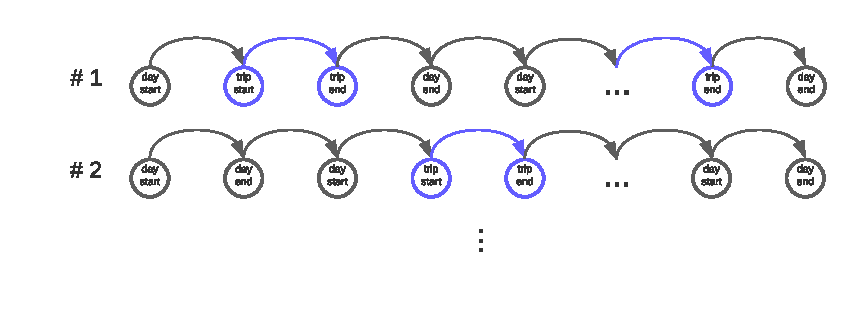
\includegraphics{Figures/trip_creation_diagram.pdf}
    \caption{Trip creation - trips marked in blue}
    \label{fig:trip_creation}
\end{figure}

Figure \ref{fig:trip_creation} shows how we extract trips and relocations from the location data.

Our rationale is that every pair of consecutive locations of one bicycle either have to be a trip, a relocation or no movement at all.
As we have the information whether a given sample is the start of a trip, the end of a trip, the start of a day and the end of the day we can easily classify each pair of consecutive locations.


We then remove all trips that are longer than one day because those are just a small amount of outliers. 
We omit all trips that exceed the speed of 25kmh, which is the limit for e-bikes in Germany [source](https://www.giant-bicycles.com/de/campaigns/wie-schnell-fahrt-ein-e-bike/21531). 
This is plausible as trips that exceed this limit are very likely to be faulty because they would need to cycle faster than the maximum speed of e-bikes without any stops during the trip. 
Also, our distance column is calculated as the distance between the start and end station, which is a lower bound on the actual distance traveled. 
Therefore, the actual distance traveled is most likely longer and the actual speed is most likely higher.

Next we aggregate the trips spatially and temporally.
For spatial aggregation we use the Hexagonal Hierarchical Geospatial Indexing System (H3) \shortcite{uber_h3_2022}, which partitions the earth into multiple hexagons of varying sizes depending on the chosen resolutions.
We use the resolutions 7, 8 and 9, where the area of one hexagons covers between \(0.1\) km\(^2\) and \(5\) km\(^2\).
Additionally, we aggregate trips across multiple time intervals of lengths 1, 2, 6 and 24 hours.


\begin{table}[h!]
    \centering
        \begin{tabular}{ c|c|c|c }
         star hexagon id & end hexagon id & time interval & \# starting trips (demand) \\ 
         \hline
         1 & 2 & 2 & 7 \\  
        \end{tabular}
    \caption{Sample of aggregated trip data}
    \label{table:aggregated_trips}
\end{table}

Table \ref{table:aggregated_trips} shows a sample of the data that results from this aggregation.
The sample states that 7 trips started during time interval 2 inside the hexagon with id 1 and ended in the hexagon with id 2.
Real h3 ids actually are in the form of Universally Unique Identifier (UUID), but we've replaced them here with numeric ids for the sake of readability.
Later we will also use an even more aggregated form of this data, which does not have end hexagon ids.



We also want to aggregate the availability of bicycles in each hexagon at a given time. 
For this purpose, we first set the availability of a given hexagon at a given time interval to the number of bicycles whose first seen locations are there.
Then we update the availability of the hexagons with each trip and relocation by subtracting from the availability in the starting hexagon and adding to the end hexagon. 
When a bicycle reaches its final location, it is subtracted from the availability.
Following this approach the availability can be expressed more formally as
\[A(h, t) = A(h, t-1) + s_t(h) - d_t(h) \delta_t^+(h) - \delta_t^-(h)\]
where \(A(h, t)\) describes the total number of available bicycles at hexagon \(h\) at time interval \(t\),
\(\delta_t^+(h)\) and \(\delta_t^-(h)\) describe the total number of incoming and outgoing trips and relocations in time interval \(t\) considering hexagon \(h\),
\(s_t(h)\) describes the number of bicycles that "spawn" (first observation) in hexagon \(h\) at time interval \(t\) and 
\(d_t(h)\) describes the number of bicycles that "vanish" (last observation) in hexagon \(h\) at time interval \(t\).



%% -------------------------------------- weather data
% TODO


%% -------------------------------------- landuse data
We further added land use data to both the trips and the hexagons in all resolutions. 
For this, we downloaded the land use data set for Leipzig from the [Kopernikus website](https://land.copernicus.eu/pan-european/corine-land-cover). 
For individual trips, we merged this on the start and end location. For hexagons, we calculated for each hexagon which percentage of the area represents which land use type. 

%% -------------------------------------- POI data
% TODO

